\documentclass[svgnames,11pt]{beamer}
\input{/home/tof/Documents/Cozy/latex-include/preambule_commun.tex}
\input{/home/tof/Documents/Cozy/latex-include/preambule_beamer.tex}
%\usepackage{pgfpages} \setbeameroption{show notes on second screen=left}
\author[]{Christophe Viroulaud}
\title{Course d'orientation\\Connexité}
\date{\framebox{\textbf{Algo 17}}}
%\logo{}
\institute{Terminale - NSI}

\begin{document}
\begin{frame}
    \titlepage
\end{frame}
\begin{frame}
    \frametitle{}

    \begin{center}
    \centering
    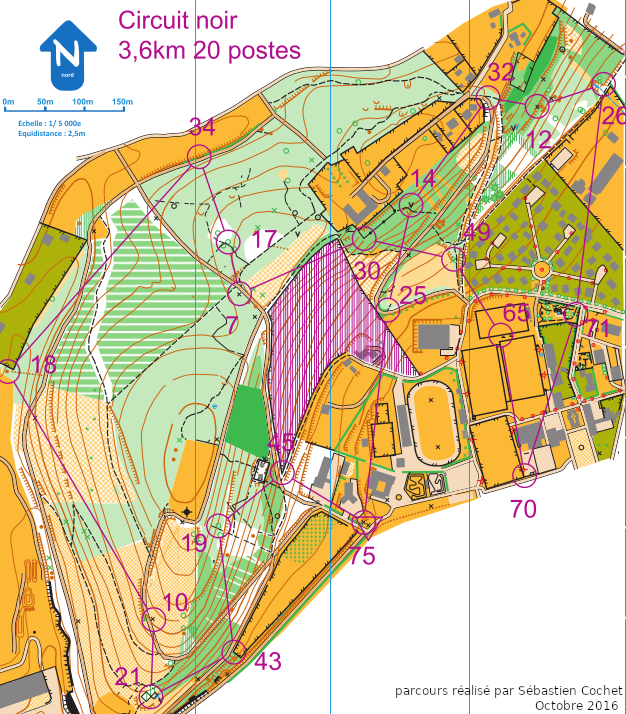
\includegraphics[width=8cm]{ressources/co-noir.png}
  
    \end{center}

\end{frame}
\begin{frame}
    \frametitle{}

    \begin{center}
        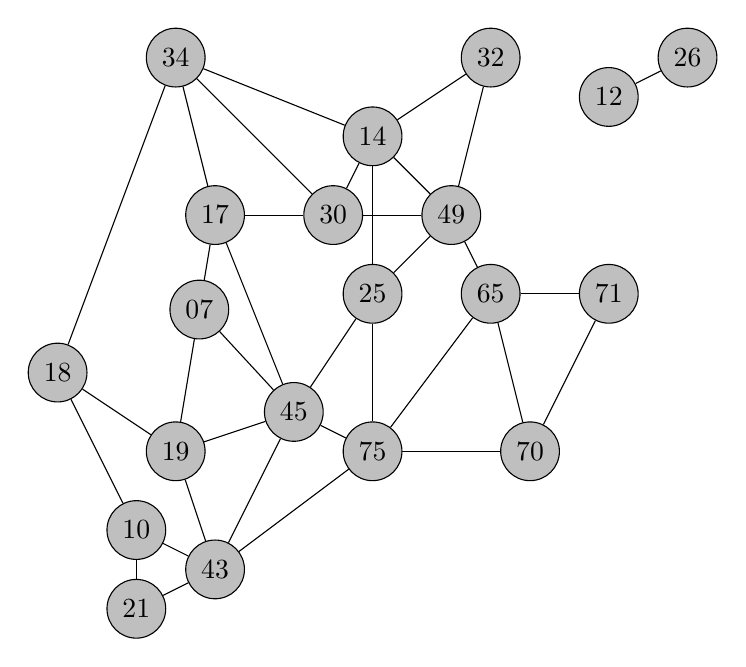
\begin{tikzpicture}
            \node[draw,circle,fill=gray!50] (21)at(0,0) {21};
            \node[draw,circle,fill=gray!50] (43)at(1,0.5) {43};
            \node[draw,circle,fill=gray!50] (10)at(0,1) {10};
            \node[draw,circle,fill=gray!50] (19)at(0.5,2) {19};
            \node[draw,circle,fill=gray!50] (45)at(2,2.5) {45};
            \node[draw,circle,fill=gray!50] (18)at(-1,3) {18};
            \node[draw,circle,fill=gray!50] (75)at(3,2) {75};
            \node[draw,circle,fill=gray!50] (70)at(5,2) {70};
            \node[draw,circle,fill=gray!50] (65)at(4.5,4) {65};
            \node[draw,circle,fill=gray!50] (71)at(6,4) {71};
            \node[draw,circle,fill=gray!50] (25)at(3,4) {25};
            \node[draw,circle,fill=gray!50] (07)at(0.8,3.8) {07};
            \node[draw,circle,fill=gray!50] (17)at(1,5) {17};
            \node[draw,circle,fill=gray!50] (30)at(2.5,5) {30};
            \node[draw,circle,fill=gray!50] (49)at(4,5) {49};
            \node[draw,circle,fill=gray!50] (14)at(3,6) {14};
            \node[draw,circle,fill=gray!50] (34)at(0.5,7) {34};
            \node[draw,circle,fill=gray!50] (32)at(4.5,7) {32};
            \node[draw,circle,fill=gray!50] (12)at(6,6.5) {12};
            \node[draw,circle,fill=gray!50] (26)at(7,7) {26};

            \draw[-,>=latex] (75) -- (45);
            \draw[-,>=latex] (75) -- (25);
            \draw[-,>=latex] (75) -- (65);
            \draw[-,>=latex] (75) -- (70);
            \draw[-,>=latex] (75) -- (43);
            \draw[-,>=latex] (45) -- (07);
            \draw[-,>=latex] (45) -- (43);
            \draw[-,>=latex] (45) -- (25);
            \draw[-,>=latex] (45) -- (19);
            \draw[-,>=latex] (45) -- (17);
            \draw[-,>=latex] (25) -- (14);
            %\draw[-,>=latex] (19) -- (10);
            \draw[-,>=latex] (19) -- (18);
            \draw[-,>=latex] (19) -- (07);
            \draw[-,>=latex] (19) -- (43);
            \draw[-,>=latex] (43) -- (10);
            \draw[-,>=latex] (43) -- (21);
            %\draw[-,>=latex] (43) -- (18);
            \draw[-,>=latex] (10) -- (21);
            \draw[-,>=latex] (10) -- (18);
            \draw[-,>=latex] (34) -- (17);
            \draw[-,>=latex] (70) -- (71);
            \draw[-,>=latex] (70) -- (65);
            \draw[-,>=latex] (49) -- (65);
            \draw[-,>=latex] (49) -- (25);
            \draw[-,>=latex] (49) -- (14);
            \draw[-,>=latex] (49) -- (30);
            \draw[-,>=latex] (49) -- (32);
            \draw[-,>=latex] (30) -- (14);
            \draw[-,>=latex] (30) -- (34);
            \draw[-,>=latex] (30) -- (17);
            \draw[-,>=latex] (14) -- (34);
            \draw[-,>=latex] (14) -- (32);
            %\draw[-,>=latex] (32) -- (12);
            \draw[-,>=latex] (12) -- (26);
            \draw[-,>=latex] (65) -- (71);
            %\draw[-,>=latex] (71) -- (26);
            \draw[-,>=latex] (18) -- (34);
            \draw[-,>=latex] (07) -- (17);

        \end{tikzpicture}
        \captionof{figure}{\centering Des chemins impraticables à cause de la météo.}
    \end{center}

\end{frame}
\begin{frame}
    \frametitle{}

    \begin{framed}
        \centering Comment vérifier si tous les sommets sont atteignables?
    \end{framed}

\end{frame}
\section{Parcours en profondeur (Depth First Search)}
\subsection{Principe}
\begin{frame}
    \frametitle{Parcours en profondeur (Depth First Search) - Principe}

    \begin{center}
        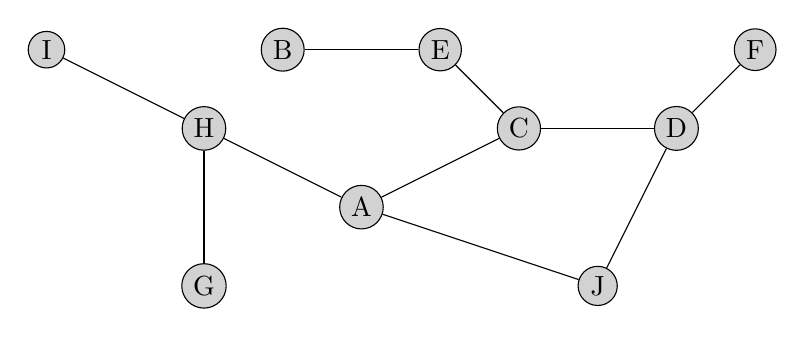
\begin{tikzpicture}
            \node[draw,circle,fill=gray!35, inner sep=2] (A)at(0,0) {A};
            \node[draw,circle,fill=gray!35, inner sep=2] (B)at(-1,2) {B};
            \node[draw,circle,fill=gray!35, inner sep=2] (C)at(2,1) {C};
            \node[draw,circle,fill=gray!35, inner sep=2] (D)at(4,1) {D};
            \node[draw,circle,fill=gray!35, inner sep=2] (E)at(1,2) {E};
            \node[draw,circle,fill=gray!35, inner sep=2] (F)at(5,2) {F};
            \node[draw,circle,fill=gray!35, inner sep=2] (G)at(-2,-1) {G};
            \node[draw,circle,fill=gray!35, inner sep=2] (H)at(-2,1) {H};
            \node[draw,circle,fill=gray!35, inner sep=2] (I)at(-4,2) {I};
            \node[draw,circle,fill=gray!35, inner sep=2] (J)at(3,-1) {J};
            \draw[-,>=latex] (E) -- (B);
            \draw[-,>=latex] (A) -- (C);
            \draw[-,>=latex] (A) -- (H);
            \draw[-,>=latex] (A) -- (J);
            \draw[-,>=latex] (H) -- (I);
            \draw[-,>=latex] (H) -- (G);
            \draw[-,>=latex] (C) -- (E);
            \draw[-,>=latex] (C) -- (D);
            %\draw[-,>=latex] (C) -- (J);
            \draw[-,>=latex] (D) -- (J);
            \draw[-,>=latex] (D) -- (F);
        \end{tikzpicture}
    \end{center}
    \begin{aretenir}[]
        Un parcours en profondeur \emph{avance} dans le graphe jusqu'à une extrémité ou un nœud déjà visité. Il revient alors à un sommet précédent qui propose un autre chemin.
    \end{aretenir}
    \note{principe parcours dans un labyrinthe}
\end{frame}
\begin{frame}
    \frametitle{}

    \begin{center}
    \centering
    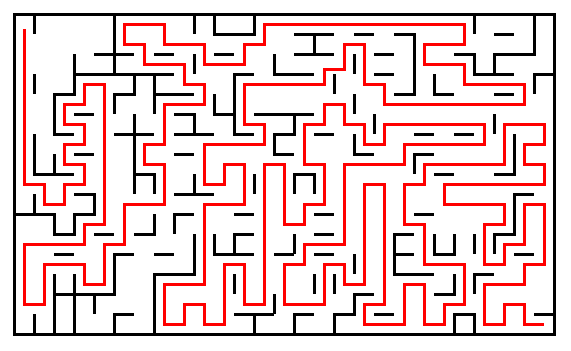
\includegraphics[width=8cm]{ressources/labyrinthe.png}
    \captionof{figure}{Parcours en profondeur dans un labyrinthe}
    \label{IMG}
    \end{center}

\end{frame}
\begin{frame}
    \frametitle{}

    \begin{center}
        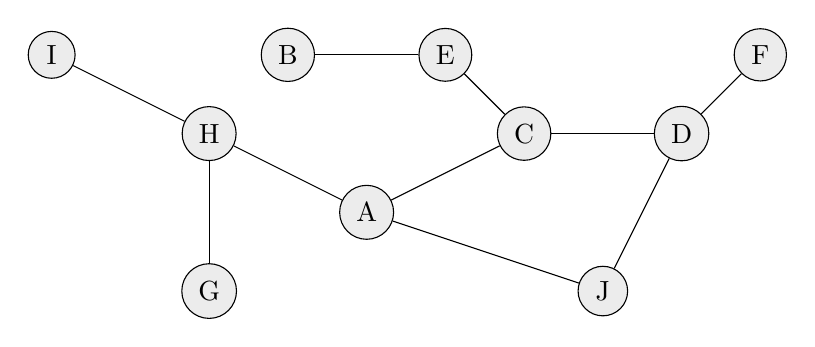
\begin{tikzpicture}
            \node[draw,circle,fill=gray!15] (A)at(0,0) {A};
            \node[draw,circle,fill=gray!15] (B)at(-1,2) {B};
            \node[draw,circle,fill=gray!15] (C)at(2,1) {C};
            \node[draw,circle,fill=gray!15] (D)at(4,1) {D};
            \node[draw,circle,fill=gray!15] (E)at(1,2) {E};
            \node[draw,circle,fill=gray!15] (F)at(5,2) {F};
            \node[draw,circle,fill=gray!15] (G)at(-2,-1) {G};
            \node[draw,circle,fill=gray!15] (H)at(-2,1) {H};
            \node[draw,circle,fill=gray!15] (I)at(-4,2) {I};
            \node[draw,circle,fill=gray!15] (J)at(3,-1) {J};
            \draw[-,>=latex] (E) -- (B);
            \draw[-,>=latex] (A) -- (C);
            \draw[-,>=latex] (A) -- (H);
            \draw[-,>=latex] (A) -- (J);
            \draw[-,>=latex] (H) -- (I);
            \draw[-,>=latex] (H) -- (G);
            \draw[-,>=latex] (C) -- (E);
            \draw[-,>=latex] (C) -- (D);
            %\draw[-,>=latex] (C) -- (J);
            \draw[-,>=latex] (D) -- (J);
            \draw[-,>=latex] (D) -- (F);
        \end{tikzpicture}
    \end{center}

\end{frame}
\begin{frame}
    \frametitle{}

    \begin{center}
        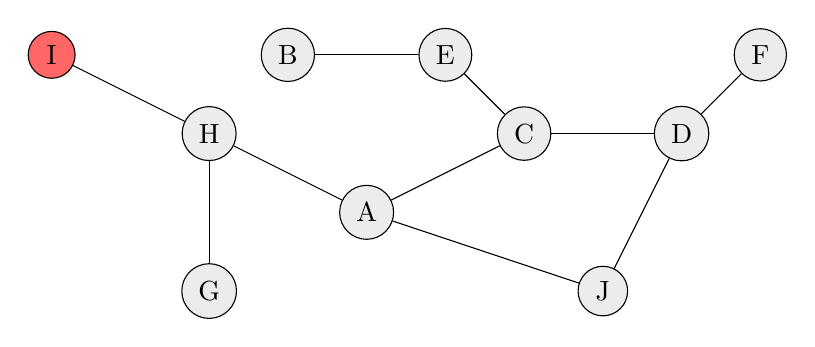
\begin{tikzpicture}
            \node[draw,circle,fill=gray!15] (A)at(0,0) {A};
            \node[draw,circle,fill=gray!15] (B)at(-1,2) {B};
            \node[draw,circle,fill=gray!15] (C)at(2,1) {C};
            \node[draw,circle,fill=gray!15] (D)at(4,1) {D};
            \node[draw,circle,fill=gray!15] (E)at(1,2) {E};
            \node[draw,circle,fill=gray!15] (F)at(5,2) {F};
            \node[draw,circle,fill=gray!15] (G)at(-2,-1) {G};
            \node[draw,circle,fill=gray!15] (H)at(-2,1) {H};
            \node[draw,circle,fill=red!60] (I)at(-4,2) {I};
            \node[draw,circle,fill=gray!15] (J)at(3,-1) {J};
            \draw[-,>=latex] (E) -- (B);
            \draw[-,>=latex] (A) -- (C);
            \draw[-,>=latex] (A) -- (H);
            \draw[-,>=latex] (A) -- (J);
            \draw[-,>=latex] (H) -- (I);
            \draw[-,>=latex] (H) -- (G);
            \draw[-,>=latex] (C) -- (E);
            \draw[-,>=latex] (C) -- (D);
            %\draw[-,>=latex] (C) -- (J);
            \draw[-,>=latex] (D) -- (J);
            \draw[-,>=latex] (D) -- (F);
        \end{tikzpicture}
    \end{center}

\end{frame}
\begin{frame}
    \frametitle{}

    \begin{center}
        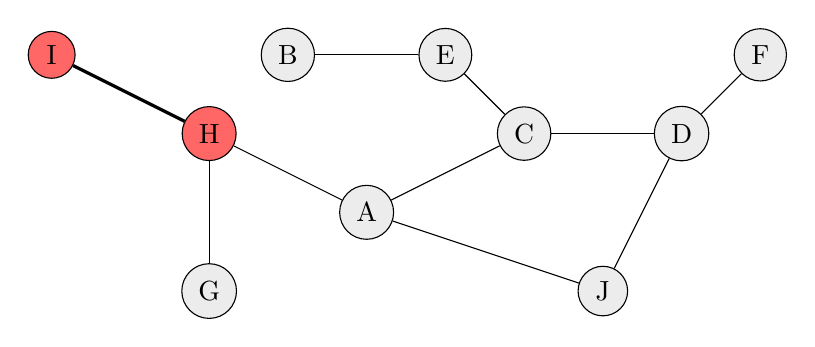
\begin{tikzpicture}
            \node[draw,circle,fill=gray!15] (A)at(0,0) {A};
            \node[draw,circle,fill=gray!15] (B)at(-1,2) {B};
            \node[draw,circle,fill=gray!15] (C)at(2,1) {C};
            \node[draw,circle,fill=gray!15] (D)at(4,1) {D};
            \node[draw,circle,fill=gray!15] (E)at(1,2) {E};
            \node[draw,circle,fill=gray!15] (F)at(5,2) {F};
            \node[draw,circle,fill=gray!15] (G)at(-2,-1) {G};
            \node[draw,circle,fill=red!60] (H)at(-2,1) {H};
            \node[draw,circle,fill=red!60] (I)at(-4,2) {I};
            \node[draw,circle,fill=gray!15] (J)at(3,-1) {J};
            \draw[-,>=latex] (E) -- (B);
            \draw[-,>=latex] (A) -- (C);
            \draw[-,>=latex] (A) -- (H);
            \draw[-,>=latex] (A) -- (J);
            \draw[-,>=latex,very thick] (H) -- (I);
            \draw[-,>=latex] (H) -- (G);
            \draw[-,>=latex] (C) -- (E);
            \draw[-,>=latex] (C) -- (D);
            %\draw[-,>=latex] (C) -- (J);
            \draw[-,>=latex] (D) -- (J);
            \draw[-,>=latex] (D) -- (F);
        \end{tikzpicture}
    \end{center}

\end{frame}
\begin{frame}
    \frametitle{}

    \begin{center}
        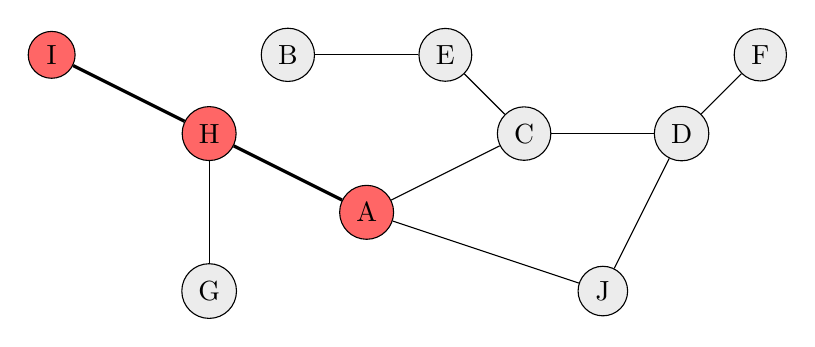
\begin{tikzpicture}
            \node[draw,circle,fill=red!60] (A)at(0,0) {A};
            \node[draw,circle,fill=gray!15] (B)at(-1,2) {B};
            \node[draw,circle,fill=gray!15] (C)at(2,1) {C};
            \node[draw,circle,fill=gray!15] (D)at(4,1) {D};
            \node[draw,circle,fill=gray!15] (E)at(1,2) {E};
            \node[draw,circle,fill=gray!15] (F)at(5,2) {F};
            \node[draw,circle,fill=gray!15] (G)at(-2,-1) {G};
            \node[draw,circle,fill=red!60] (H)at(-2,1) {H};
            \node[draw,circle,fill=red!60] (I)at(-4,2) {I};
            \node[draw,circle,fill=gray!15] (J)at(3,-1) {J};
            \draw[-,>=latex] (E) -- (B);
            \draw[-,>=latex] (A) -- (C);
            \draw[-,>=latex,very thick] (A) -- (H);
            \draw[-,>=latex] (A) -- (J);
            \draw[-,>=latex,very thick] (H) -- (I);
            \draw[-,>=latex] (H) -- (G);
            \draw[-,>=latex] (C) -- (E);
            \draw[-,>=latex] (C) -- (D);
            %\draw[-,>=latex] (C) -- (J);
            \draw[-,>=latex] (D) -- (J);
            \draw[-,>=latex] (D) -- (F);
        \end{tikzpicture}
    \end{center}

\end{frame}
\begin{frame}
    \frametitle{}

    \begin{center}
        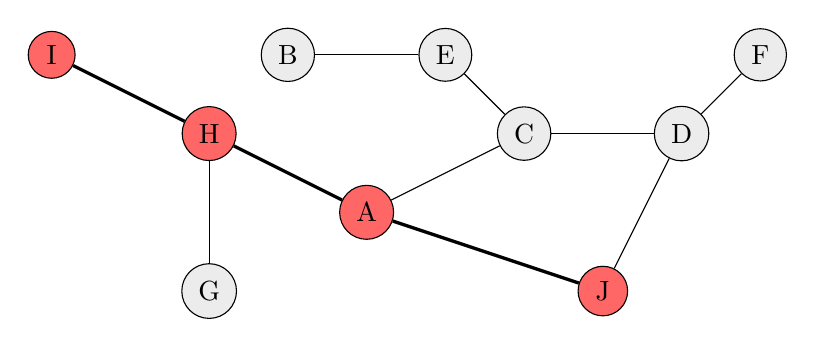
\begin{tikzpicture}
            \node[draw,circle,fill=red!60] (A)at(0,0) {A};
            \node[draw,circle,fill=gray!15] (B)at(-1,2) {B};
            \node[draw,circle,fill=gray!15] (C)at(2,1) {C};
            \node[draw,circle,fill=gray!15] (D)at(4,1) {D};
            \node[draw,circle,fill=gray!15] (E)at(1,2) {E};
            \node[draw,circle,fill=gray!15] (F)at(5,2) {F};
            \node[draw,circle,fill=gray!15] (G)at(-2,-1) {G};
            \node[draw,circle,fill=red!60] (H)at(-2,1) {H};
            \node[draw,circle,fill=red!60] (I)at(-4,2) {I};
            \node[draw,circle,fill=red!60] (J)at(3,-1) {J};
            \draw[-,>=latex] (E) -- (B);
            \draw[-,>=latex] (A) -- (C);
            \draw[-,>=latex,very thick] (A) -- (H);
            \draw[-,>=latex,very thick] (A) -- (J);
            \draw[-,>=latex,very thick] (H) -- (I);
            \draw[-,>=latex] (H) -- (G);
            \draw[-,>=latex] (C) -- (E);
            \draw[-,>=latex] (C) -- (D);
            %\draw[-,>=latex] (C) -- (J);
            \draw[-,>=latex] (D) -- (J);
            \draw[-,>=latex] (D) -- (F);
        \end{tikzpicture}
    \end{center}

\end{frame}
\begin{frame}
    \frametitle{}

    \begin{center}
        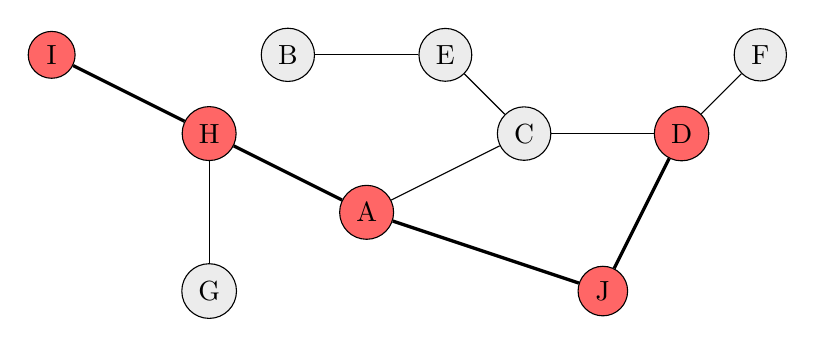
\begin{tikzpicture}
            \node[draw,circle,fill=red!60] (A)at(0,0) {A};
            \node[draw,circle,fill=gray!15] (B)at(-1,2) {B};
            \node[draw,circle,fill=gray!15] (C)at(2,1) {C};
            \node[draw,circle,fill=red!60] (D)at(4,1) {D};
            \node[draw,circle,fill=gray!15] (E)at(1,2) {E};
            \node[draw,circle,fill=gray!15] (F)at(5,2) {F};
            \node[draw,circle,fill=gray!15] (G)at(-2,-1) {G};
            \node[draw,circle,fill=red!60] (H)at(-2,1) {H};
            \node[draw,circle,fill=red!60] (I)at(-4,2) {I};
            \node[draw,circle,fill=red!60] (J)at(3,-1) {J};
            \draw[-,>=latex] (E) -- (B);
            \draw[-,>=latex] (A) -- (C);
            \draw[-,>=latex,very thick] (A) -- (H);
            \draw[-,>=latex,very thick] (A) -- (J);
            \draw[-,>=latex,very thick] (H) -- (I);
            \draw[-,>=latex] (H) -- (G);
            \draw[-,>=latex] (C) -- (E);
            \draw[-,>=latex] (C) -- (D);
            %\draw[-,>=latex] (C) -- (J);
            \draw[-,>=latex,very thick] (D) -- (J);
            \draw[-,>=latex] (D) -- (F);
        \end{tikzpicture}
    \end{center}

\end{frame}
\begin{frame}
    \frametitle{}

    \begin{center}
        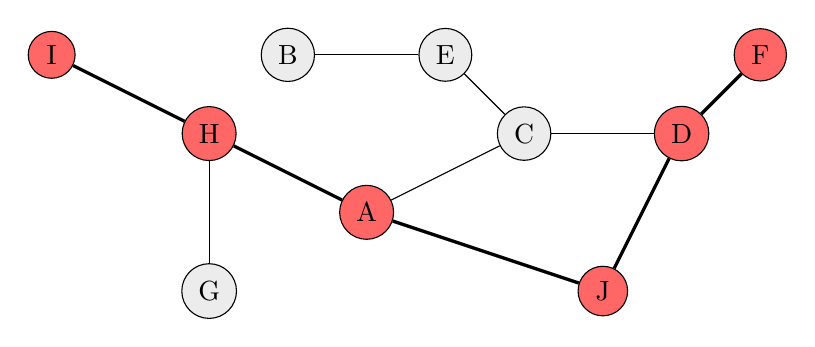
\begin{tikzpicture}
            \node[draw,circle,fill=red!60] (A)at(0,0) {A};
            \node[draw,circle,fill=gray!15] (B)at(-1,2) {B};
            \node[draw,circle,fill=gray!15] (C)at(2,1) {C};
            \node[draw,circle,fill=red!60] (D)at(4,1) {D};
            \node[draw,circle,fill=gray!15] (E)at(1,2) {E};
            \node[draw,circle,fill=red!60] (F)at(5,2) {F};
            \node[draw,circle,fill=gray!15] (G)at(-2,-1) {G};
            \node[draw,circle,fill=red!60] (H)at(-2,1) {H};
            \node[draw,circle,fill=red!60] (I)at(-4,2) {I};
            \node[draw,circle,fill=red!60] (J)at(3,-1) {J};
            \draw[-,>=latex] (E) -- (B);
            \draw[-,>=latex] (A) -- (C);
            \draw[-,>=latex,very thick] (A) -- (H);
            \draw[-,>=latex,very thick] (A) -- (J);
            \draw[-,>=latex,very thick] (H) -- (I);
            \draw[-,>=latex] (H) -- (G);
            \draw[-,>=latex] (C) -- (E);
            \draw[-,>=latex] (C) -- (D);
            %\draw[-,>=latex] (C) -- (J);
            \draw[-,>=latex,very thick] (D) -- (J);
            \draw[-,>=latex,very thick] (D) -- (F);
        \end{tikzpicture}
        \captionof{figure}{Retour au nœud précédent}
    \end{center}

\end{frame}
\begin{frame}
    \frametitle{}

    \begin{center}
        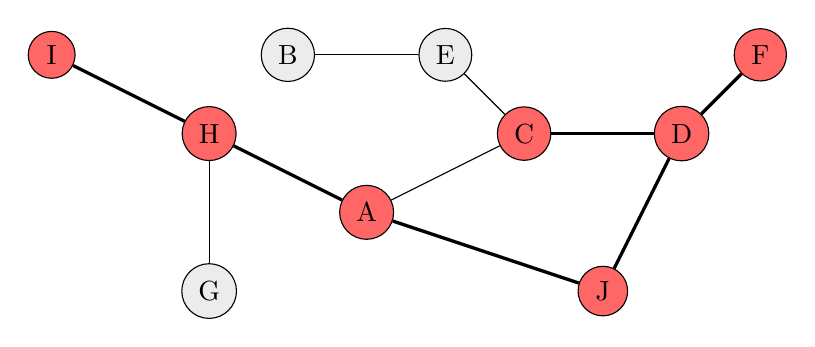
\begin{tikzpicture}
            \node[draw,circle,fill=red!60] (A)at(0,0) {A};
            \node[draw,circle,fill=gray!15] (B)at(-1,2) {B};
            \node[draw,circle,fill=red!60] (C)at(2,1) {C};
            \node[draw,circle,fill=red!60] (D)at(4,1) {D};
            \node[draw,circle,fill=gray!15] (E)at(1,2) {E};
            \node[draw,circle,fill=red!60] (F)at(5,2) {F};
            \node[draw,circle,fill=gray!15] (G)at(-2,-1) {G};
            \node[draw,circle,fill=red!60] (H)at(-2,1) {H};
            \node[draw,circle,fill=red!60] (I)at(-4,2) {I};
            \node[draw,circle,fill=red!60] (J)at(3,-1) {J};
            \draw[-,>=latex] (E) -- (B);
            \draw[-,>=latex] (A) -- (C);
            \draw[-,>=latex,very thick] (A) -- (H);
            \draw[-,>=latex,very thick] (A) -- (J);
            \draw[-,>=latex,very thick] (H) -- (I);
            \draw[-,>=latex] (H) -- (G);
            \draw[-,>=latex] (C) -- (E);
            \draw[-,>=latex,very thick] (C) -- (D);
            %\draw[-,>=latex] (C) -- (J);
            \draw[-,>=latex,very thick] (D) -- (J);
            \draw[-,>=latex,very thick] (D) -- (F);
        \end{tikzpicture}
    \end{center}

\end{frame}
\begin{frame}
    \frametitle{}

    \begin{center}
        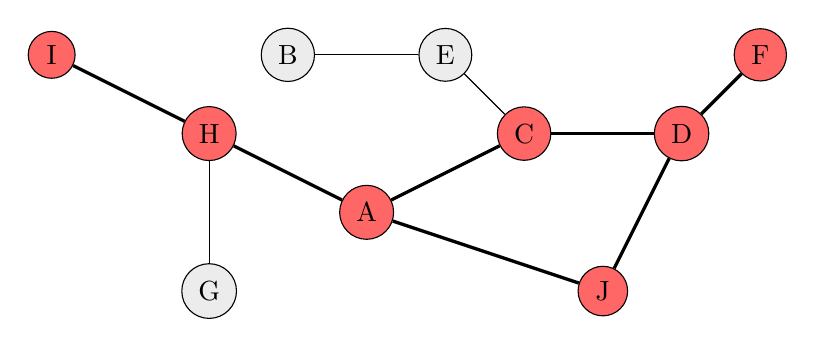
\begin{tikzpicture}
            \node[draw,circle,fill=red!60] (A)at(0,0) {A};
            \node[draw,circle,fill=gray!15] (B)at(-1,2) {B};
            \node[draw,circle,fill=red!60] (C)at(2,1) {C};
            \node[draw,circle,fill=red!60] (D)at(4,1) {D};
            \node[draw,circle,fill=gray!15] (E)at(1,2) {E};
            \node[draw,circle,fill=red!60] (F)at(5,2) {F};
            \node[draw,circle,fill=gray!15] (G)at(-2,-1) {G};
            \node[draw,circle,fill=red!60] (H)at(-2,1) {H};
            \node[draw,circle,fill=red!60] (I)at(-4,2) {I};
            \node[draw,circle,fill=red!60] (J)at(3,-1) {J};
            \draw[-,>=latex] (E) -- (B);
            \draw[-,>=latex,very thick] (A) -- (C);
            \draw[-,>=latex,very thick] (A) -- (H);
            \draw[-,>=latex,very thick] (A) -- (J);
            \draw[-,>=latex,very thick] (H) -- (I);
            \draw[-,>=latex] (H) -- (G);
            \draw[-,>=latex] (C) -- (E);
            \draw[-,>=latex,very thick] (C) -- (D);
            %\draw[-,>=latex] (C) -- (J);
            \draw[-,>=latex,very thick] (D) -- (J);
            \draw[-,>=latex,very thick] (D) -- (F);
        \end{tikzpicture}
        \captionof{figure}{\textbf{\texttt{A}} est déjà visité.}
    \end{center}

\end{frame}
\begin{frame}
    \frametitle{}


    \begin{center}
        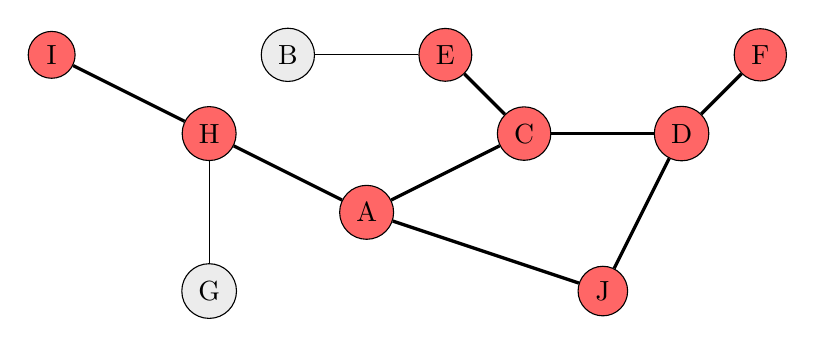
\begin{tikzpicture}
            \node[draw,circle,fill=red!60] (A)at(0,0) {A};
            \node[draw,circle,fill=gray!15] (B)at(-1,2) {B};
            \node[draw,circle,fill=red!60] (C)at(2,1) {C};
            \node[draw,circle,fill=red!60] (D)at(4,1) {D};
            \node[draw,circle,fill=red!60] (E)at(1,2) {E};
            \node[draw,circle,fill=red!60] (F)at(5,2) {F};
            \node[draw,circle,fill=gray!15] (G)at(-2,-1) {G};
            \node[draw,circle,fill=red!60] (H)at(-2,1) {H};
            \node[draw,circle,fill=red!60] (I)at(-4,2) {I};
            \node[draw,circle,fill=red!60] (J)at(3,-1) {J};
            \draw[-,>=latex] (E) -- (B);
            \draw[-,>=latex,very thick] (A) -- (C);
            \draw[-,>=latex,very thick] (A) -- (H);
            \draw[-,>=latex,very thick] (A) -- (J);
            \draw[-,>=latex,very thick] (H) -- (I);
            \draw[-,>=latex] (H) -- (G);
            \draw[-,>=latex,very thick] (C) -- (E);
            \draw[-,>=latex,very thick] (C) -- (D);
            %\draw[-,>=latex] (C) -- (J);
            \draw[-,>=latex,very thick] (D) -- (J);
            \draw[-,>=latex,very thick] (D) -- (F);
        \end{tikzpicture}
    \end{center}

\end{frame}
\begin{frame}
    \frametitle{}

    \begin{center}
        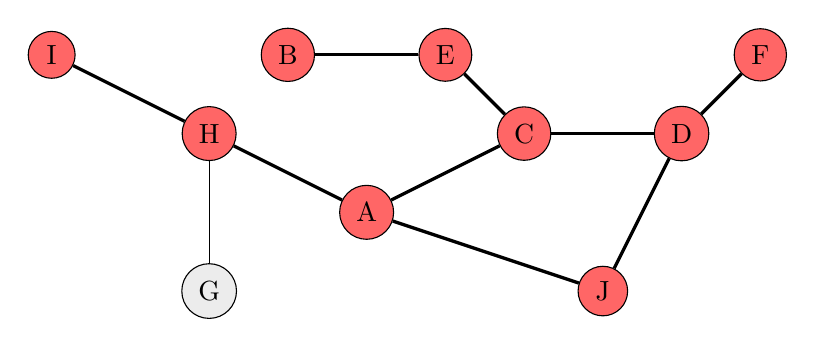
\begin{tikzpicture}
            \node[draw,circle,fill=red!60] (A)at(0,0) {A};
            \node[draw,circle,fill=red!60] (B)at(-1,2) {B};
            \node[draw,circle,fill=red!60] (C)at(2,1) {C};
            \node[draw,circle,fill=red!60] (D)at(4,1) {D};
            \node[draw,circle,fill=red!60] (E)at(1,2) {E};
            \node[draw,circle,fill=red!60] (F)at(5,2) {F};
            \node[draw,circle,fill=gray!15] (G)at(-2,-1) {G};
            \node[draw,circle,fill=red!60] (H)at(-2,1) {H};
            \node[draw,circle,fill=red!60] (I)at(-4,2) {I};
            \node[draw,circle,fill=red!60] (J)at(3,-1) {J};
            \draw[-,>=latex,very thick] (E) -- (B);
            \draw[-,>=latex,very thick] (A) -- (C);
            \draw[-,>=latex,very thick] (A) -- (H);
            \draw[-,>=latex,very thick] (A) -- (J);
            \draw[-,>=latex,very thick] (H) -- (I);
            \draw[-,>=latex] (H) -- (G);
            \draw[-,>=latex,very thick] (C) -- (E);
            \draw[-,>=latex,very thick] (C) -- (D);
            %\draw[-,>=latex] (C) -- (J);
            \draw[-,>=latex,very thick] (D) -- (J);
            \draw[-,>=latex,very thick] (D) -- (F);
        \end{tikzpicture}
    \end{center}

\end{frame}
\begin{frame}
    \frametitle{}

    \begin{center}
        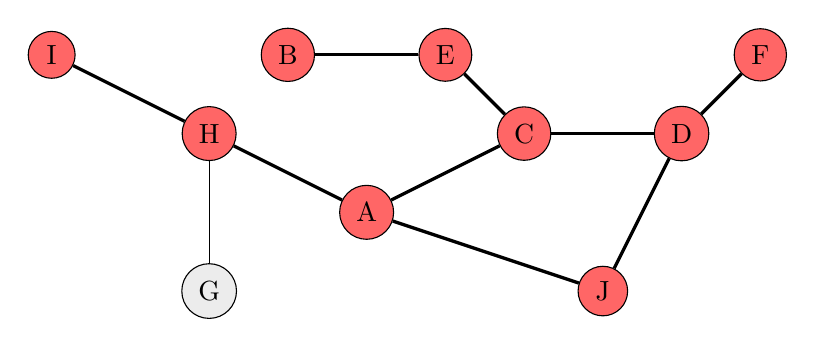
\begin{tikzpicture}
            \node[draw,circle,fill=red!60] (A)at(0,0) {A};
            \node[draw,circle,fill=red!60] (B)at(-1,2) {B};
            \node[draw,circle,fill=red!60] (C)at(2,1) {C};
            \node[draw,circle,fill=red!60] (D)at(4,1) {D};
            \node[draw,circle,fill=red!60] (E)at(1,2) {E};
            \node[draw,circle,fill=red!60] (F)at(5,2) {F};
            \node[draw,circle,fill=gray!15] (G)at(-2,-1) {G};
            \node[draw,circle,fill=red!60] (H)at(-2,1) {H};
            \node[draw,circle,fill=red!60] (I)at(-4,2) {I};
            \node[draw,circle,fill=red!60] (J)at(3,-1) {J};
            \draw[-,>=latex,very thick] (E) -- (B);
            \draw[-,>=latex,very thick] (A) -- (C);
            \draw[-,>=latex,very thick] (A) -- (H);
            \draw[-,>=latex,very thick] (A) -- (J);
            \draw[-,>=latex,very thick] (H) -- (I);
            \draw[-,>=latex] (H) -- (G);
            \draw[-,>=latex,very thick] (C) -- (E);
            \draw[-,>=latex,very thick] (C) -- (D);
            %\draw[-,>=latex] (C) -- (J);
            \draw[-,>=latex,very thick] (D) -- (J);
            \draw[-,>=latex,very thick] (D) -- (F);
        \end{tikzpicture}
        \captionof{figure}{Retour au nœud précédent}
    \end{center}

\end{frame}
\begin{frame}
    \frametitle{}

    \begin{center}
        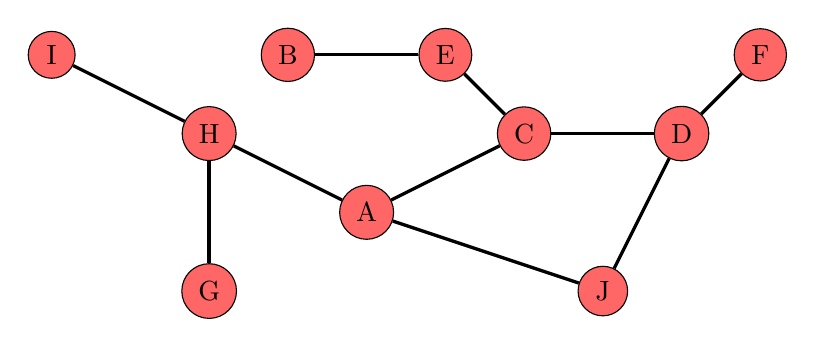
\begin{tikzpicture}
            \node[draw,circle,fill=red!60] (A)at(0,0) {A};
            \node[draw,circle,fill=red!60] (B)at(-1,2) {B};
            \node[draw,circle,fill=red!60] (C)at(2,1) {C};
            \node[draw,circle,fill=red!60] (D)at(4,1) {D};
            \node[draw,circle,fill=red!60] (E)at(1,2) {E};
            \node[draw,circle,fill=red!60] (F)at(5,2) {F};
            \node[draw,circle,fill=red!60] (G)at(-2,-1) {G};
            \node[draw,circle,fill=red!60] (H)at(-2,1) {H};
            \node[draw,circle,fill=red!60] (I)at(-4,2) {I};
            \node[draw,circle,fill=red!60] (J)at(3,-1) {J};
            \draw[-,>=latex,very thick] (E) -- (B);
            \draw[-,>=latex,very thick] (A) -- (C);
            \draw[-,>=latex,very thick] (A) -- (H);
            \draw[-,>=latex,very thick] (A) -- (J);
            \draw[-,>=latex,very thick] (H) -- (I);
            \draw[-,>=latex,very thick] (H) -- (G);
            \draw[-,>=latex,very thick] (C) -- (E);
            \draw[-,>=latex,very thick] (C) -- (D);
            %\draw[-,>=latex] (C) -- (J);
            \draw[-,>=latex,very thick] (D) -- (J);
            \draw[-,>=latex,very thick] (D) -- (F);
        \end{tikzpicture}
        \captionof{figure}{Fin du parcours}
    \end{center}

\end{frame}
\subsection{Complexité}
\begin{frame}
    \frametitle{Complexité}
    \begin{center}
        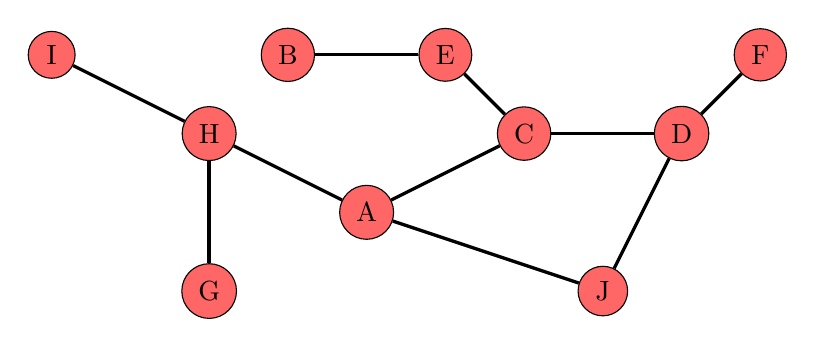
\begin{tikzpicture}
            \node[draw,circle,fill=red!60] (A)at(0,0) {A};
            \node[draw,circle,fill=red!60] (B)at(-1,2) {B};
            \node[draw,circle,fill=red!60] (C)at(2,1) {C};
            \node[draw,circle,fill=red!60] (D)at(4,1) {D};
            \node[draw,circle,fill=red!60] (E)at(1,2) {E};
            \node[draw,circle,fill=red!60] (F)at(5,2) {F};
            \node[draw,circle,fill=red!60] (G)at(-2,-1) {G};
            \node[draw,circle,fill=red!60] (H)at(-2,1) {H};
            \node[draw,circle,fill=red!60] (I)at(-4,2) {I};
            \node[draw,circle,fill=red!60] (J)at(3,-1) {J};
            \draw[-,>=latex,very thick] (E) -- (B);
            \draw[-,>=latex,very thick] (A) -- (C);
            \draw[-,>=latex,very thick] (A) -- (H);
            \draw[-,>=latex,very thick] (A) -- (J);
            \draw[-,>=latex,very thick] (H) -- (I);
            \draw[-,>=latex,very thick] (H) -- (G);
            \draw[-,>=latex,very thick] (C) -- (E);
            \draw[-,>=latex,very thick] (C) -- (D);
            %\draw[-,>=latex] (C) -- (J);
            \draw[-,>=latex,very thick] (D) -- (J);
            \draw[-,>=latex,very thick] (D) -- (F);
        \end{tikzpicture}
        \captionof{figure}{Fin du parcours}
    \end{center}
    \begin{aretenir}[]
    \begin{itemize}
        \item<1-> On ne parcourt chaque arête qu'une seule fois. 
        \item<2-> On ne marque chaque nœud qu'une fois.
        \item<3-> La complexité du parcours en profondeur dépend du nombre de nœuds et du nombre d'arêtes du graphe.
    \end{itemize}
    \end{aretenir}
    

\end{frame}
\subsection{Implémentation}
\begin{frame}
    \frametitle{Implémentation}

    \begin{aretenir}[]
    Le parcours en profondeur est naturellement récursif. On choisit un nœud de départ pour commencer le parcours, puis:
    \begin{itemize}
        \item Si le nœud n'est pas déjà visité:
        \begin{itemize}
            \item faire quelque chose avec le nœud (afficher\dots)
            \item le marquer \emph{visité},
            \item pour tous les nœuds voisins:
            \begin{itemize}
                \item effectuer le parcours récursivement depuis le voisin sélectionné.
            \end{itemize}
        \end{itemize}
    \end{itemize}
    \end{aretenir}

\end{frame}
\begin{frame}
    \frametitle{}
    \begin{center}
        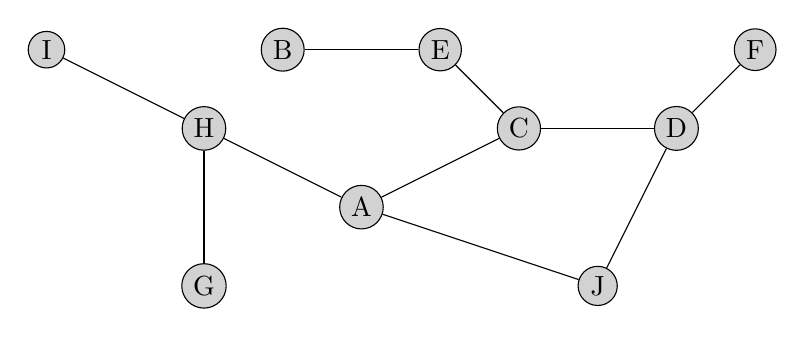
\begin{tikzpicture}
            \node[draw,circle,fill=gray!35, inner sep=2] (A)at(0,0) {A};
            \node[draw,circle,fill=gray!35, inner sep=2] (B)at(-1,2) {B};
            \node[draw,circle,fill=gray!35, inner sep=2] (C)at(2,1) {C};
            \node[draw,circle,fill=gray!35, inner sep=2] (D)at(4,1) {D};
            \node[draw,circle,fill=gray!35, inner sep=2] (E)at(1,2) {E};
            \node[draw,circle,fill=gray!35, inner sep=2] (F)at(5,2) {F};
            \node[draw,circle,fill=gray!35, inner sep=2] (G)at(-2,-1) {G};
            \node[draw,circle,fill=gray!35, inner sep=2] (H)at(-2,1) {H};
            \node[draw,circle,fill=gray!35, inner sep=2] (I)at(-4,2) {I};
            \node[draw,circle,fill=gray!35, inner sep=2] (J)at(3,-1) {J};
            \draw[-,>=latex] (E) -- (B);
            \draw[-,>=latex] (A) -- (C);
            \draw[-,>=latex] (A) -- (H);
            \draw[-,>=latex] (A) -- (J);
            \draw[-,>=latex] (H) -- (I);
            \draw[-,>=latex] (H) -- (G);
            \draw[-,>=latex] (C) -- (E);
            \draw[-,>=latex] (C) -- (D);
            %\draw[-,>=latex] (C) -- (J);
            \draw[-,>=latex] (D) -- (J);
            \draw[-,>=latex] (D) -- (F);
        \end{tikzpicture}
    \end{center}
    \begin{activite}
    \begin{enumerate}
        \item Construire le dictionnaire d'adjacence du graphe.
        \item Écrire la fonction récursive \textbf{\texttt{profondeur(graphe: dict, noeud: str, visites: list) $\rightarrow$ None}} qui effectue un parcours en profondeur du \textbf{\texttt{graphe}}. À chaque appel, le nœud traversé sera affiché dans la console.
    \end{enumerate}
    \end{activite}

\end{frame}
\begin{frame}[fragile]
    \frametitle{Correction}

    \begin{center}
    \begin{lstlisting}[language=Python , basicstyle=\ttfamily\small, xleftmargin=2em, xrightmargin=2em]
graphe = {  "A": ["C", "H", "J"],
            "B": ["E"],
            "C": ["A", "D", "E"],
            "D": ["C", "F", "J"],
            "E": ["B", "C"],
            "F": ["D"],
            "G": ["H"],
            "H": ["A", "G", "I"],
            "I": ["H"],
            "J": ["A", "D"]}
\end{lstlisting}
    \end{center}

\end{frame}
\begin{frame}[fragile]
    \frametitle{}

  \begin{center}
    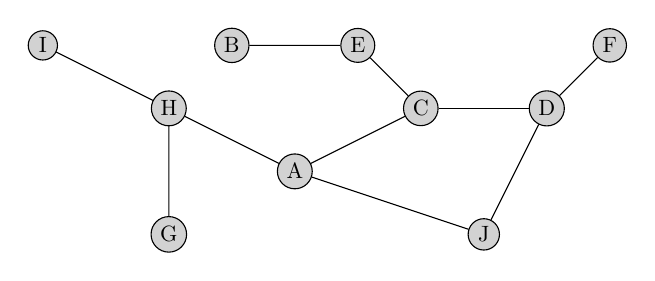
\begin{tikzpicture}[scale=0.8, transform shape]
        \node[draw,circle,fill=gray!35, inner sep=2] (A)at(0,0) {A};
        \node[draw,circle,fill=gray!35, inner sep=2] (B)at(-1,2) {B};
        \node[draw,circle,fill=gray!35, inner sep=2] (C)at(2,1) {C};
        \node[draw,circle,fill=gray!35, inner sep=2] (D)at(4,1) {D};
        \node[draw,circle,fill=gray!35, inner sep=2] (E)at(1,2) {E};
        \node[draw,circle,fill=gray!35, inner sep=2] (F)at(5,2) {F};
        \node[draw,circle,fill=gray!35, inner sep=2] (G)at(-2,-1) {G};
        \node[draw,circle,fill=gray!35, inner sep=2] (H)at(-2,1) {H};
        \node[draw,circle,fill=gray!35, inner sep=2] (I)at(-4,2) {I};
        \node[draw,circle,fill=gray!35, inner sep=2] (J)at(3,-1) {J};
        \draw[-,>=latex] (E) -- (B);
        \draw[-,>=latex] (A) -- (C);
        \draw[-,>=latex] (A) -- (H);
        \draw[-,>=latex] (A) -- (J);
        \draw[-,>=latex] (H) -- (I);
        \draw[-,>=latex] (H) -- (G);
        \draw[-,>=latex] (C) -- (E);
        \draw[-,>=latex] (C) -- (D);
        %\draw[-,>=latex] (C) -- (J);
        \draw[-,>=latex] (D) -- (J);
        \draw[-,>=latex] (D) -- (F);
    \end{tikzpicture}
  \begin{lstlisting}[language=Python , basicstyle=\ttfamily\small, xleftmargin=0.2em, xrightmargin=-6.5em]
def profondeur(graphe: dict, noeud: str, visites: list) -> None:
    if noeud not in visites:
        # on fait quelque chose avec le noeud
        print(noeud)
        visites.append(noeud)
        for voisin in graphe[noeud]:
            profondeur(graphe, voisin, visites)
\end{lstlisting}
  \end{center}  
\begin{center}
\begin{lstlisting}[language=Python , basicstyle=\ttfamily\small, xleftmargin=2em, xrightmargin=2em]
>>> profondeur(graphe, "I", [])
I H A C D F J E B G
\end{lstlisting}
\end{center}
\end{frame}
\begin{frame}[fragile]
    \frametitle{}

\begin{center}
    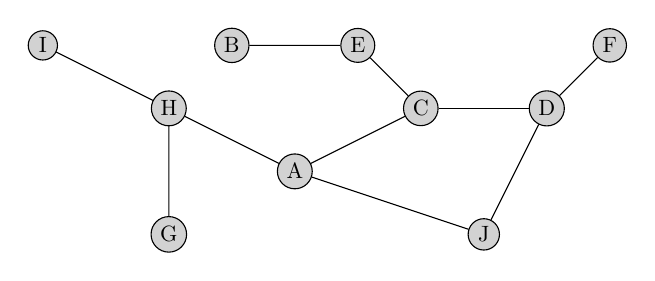
\begin{tikzpicture}[scale=0.8, transform shape]
        \node[draw,circle,fill=gray!35, inner sep=2] (A)at(0,0) {A};
        \node[draw,circle,fill=gray!35, inner sep=2] (B)at(-1,2) {B};
        \node[draw,circle,fill=gray!35, inner sep=2] (C)at(2,1) {C};
        \node[draw,circle,fill=gray!35, inner sep=2] (D)at(4,1) {D};
        \node[draw,circle,fill=gray!35, inner sep=2] (E)at(1,2) {E};
        \node[draw,circle,fill=gray!35, inner sep=2] (F)at(5,2) {F};
        \node[draw,circle,fill=gray!35, inner sep=2] (G)at(-2,-1) {G};
        \node[draw,circle,fill=gray!35, inner sep=2] (H)at(-2,1) {H};
        \node[draw,circle,fill=gray!35, inner sep=2] (I)at(-4,2) {I};
        \node[draw,circle,fill=gray!35, inner sep=2] (J)at(3,-1) {J};
        \draw[-,>=latex] (E) -- (B);
        \draw[-,>=latex] (A) -- (C);
        \draw[-,>=latex] (A) -- (H);
        \draw[-,>=latex] (A) -- (J);
        \draw[-,>=latex] (H) -- (I);
        \draw[-,>=latex] (H) -- (G);
        \draw[-,>=latex] (C) -- (E);
        \draw[-,>=latex] (C) -- (D);
        %\draw[-,>=latex] (C) -- (J);
        \draw[-,>=latex] (D) -- (J);
        \draw[-,>=latex] (D) -- (F);
    \end{tikzpicture}

\begin{lstlisting}[language=Python , basicstyle=\ttfamily\small, xleftmargin=2em, xrightmargin=2em]
    if noeud not in visites:
\end{lstlisting}
\end{center} 
\begin{aretenir}[Observations]
    \begin{itemize}
        \item<1-> Cette vérification garantit que chaque nœud et chaque arête ne sont visités qu'une fois.
        \item<2-> Cependant l'implémentation masque un coût: le parcours du tableau \textbf{\texttt{visites}}.
    \end{itemize} 
\end{aretenir}
\end{frame}
\section{Connexité}
\subsection{Définition}
\begin{frame}
    \frametitle{Connexité - Définition}
\begin{aretenir}[]
    Dans un graphe, une \textbf{chaîne} reliant deux sommets x et y est une suite d'arêtes consécutives reliant x à y.
\end{aretenir}
\begin{center}
    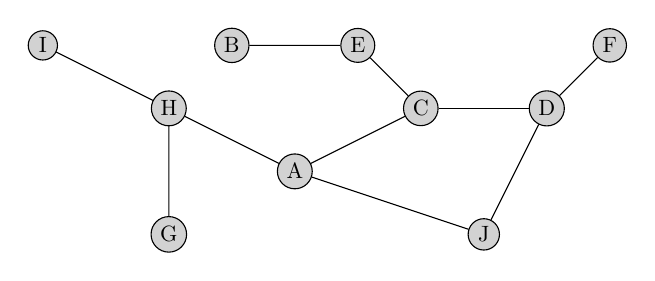
\begin{tikzpicture}[scale=0.8, transform shape]
        \node[draw,circle,fill=gray!35, inner sep=2] (A)at(0,0) {A};
        \node[draw,circle,fill=gray!35, inner sep=2] (B)at(-1,2) {B};
        \node[draw,circle,fill=gray!35, inner sep=2] (C)at(2,1) {C};
        \node[draw,circle,fill=gray!35, inner sep=2] (D)at(4,1) {D};
        \node[draw,circle,fill=gray!35, inner sep=2] (E)at(1,2) {E};
        \node[draw,circle,fill=gray!35, inner sep=2] (F)at(5,2) {F};
        \node[draw,circle,fill=gray!35, inner sep=2] (G)at(-2,-1) {G};
        \node[draw,circle,fill=gray!35, inner sep=2] (H)at(-2,1) {H};
        \node[draw,circle,fill=gray!35, inner sep=2] (I)at(-4,2) {I};
        \node[draw,circle,fill=gray!35, inner sep=2] (J)at(3,-1) {J};
        \draw[-,>=latex] (E) -- (B);
        \draw[-,>=latex] (A) -- (C);
        \draw[-,>=latex] (A) -- (H);
        \draw[-,>=latex] (A) -- (J);
        \draw[-,>=latex] (H) -- (I);
        \draw[-,>=latex] (H) -- (G);
        \draw[-,>=latex] (C) -- (E);
        \draw[-,>=latex] (C) -- (D);
        %\draw[-,>=latex] (C) -- (J);
        \draw[-,>=latex] (D) -- (J);
        \draw[-,>=latex] (D) -- (F);
    \end{tikzpicture}
\end{center}
\end{frame}
\begin{frame}
    \frametitle{Connexité - Définition}
\begin{aretenir}[]
    Dans un graphe, une \textbf{chaîne} reliant deux sommets x et y est une suite d'arêtes consécutives reliant x à y.
\end{aretenir}
    \begin{aretenir}[]
        Un graphe est \textbf{connexe} quand tout sommet peut être relié à tout autre par une chaîne.
    \end{aretenir}

\end{frame}
\subsection{Vérification de la connexité}

\begin{frame}
    \frametitle{Vérification de la connexité}

    \begin{center}
        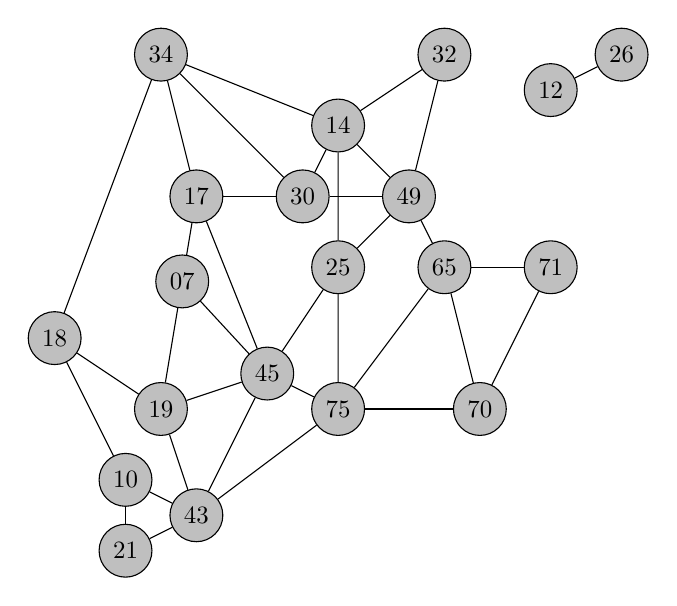
\begin{tikzpicture}[scale=0.9, transform shape]
            \node[draw,circle,fill=gray!50] (21)at(0,0) {21};
            \node[draw,circle,fill=gray!50] (43)at(1,0.5) {43};
            \node[draw,circle,fill=gray!50] (10)at(0,1) {10};
            \node[draw,circle,fill=gray!50] (19)at(0.5,2) {19};
            \node[draw,circle,fill=gray!50] (45)at(2,2.5) {45};
            \node[draw,circle,fill=gray!50] (18)at(-1,3) {18};
            \node[draw,circle,fill=gray!50] (75)at(3,2) {75};
            \node[draw,circle,fill=gray!50] (70)at(5,2) {70};
            \node[draw,circle,fill=gray!50] (65)at(4.5,4) {65};
            \node[draw,circle,fill=gray!50] (71)at(6,4) {71};
            \node[draw,circle,fill=gray!50] (25)at(3,4) {25};
            \node[draw,circle,fill=gray!50] (07)at(0.8,3.8) {07};
            \node[draw,circle,fill=gray!50] (17)at(1,5) {17};
            \node[draw,circle,fill=gray!50] (30)at(2.5,5) {30};
            \node[draw,circle,fill=gray!50] (49)at(4,5) {49};
            \node[draw,circle,fill=gray!50] (14)at(3,6) {14};
            \node[draw,circle,fill=gray!50] (34)at(0.5,7) {34};
            \node[draw,circle,fill=gray!50] (32)at(4.5,7) {32};
            \node[draw,circle,fill=gray!50] (12)at(6,6.5) {12};
            \node[draw,circle,fill=gray!50] (26)at(7,7) {26};

            \draw[-,>=latex] (75) -- (45);
            \draw[-,>=latex] (75) -- (25);
            \draw[-,>=latex] (75) -- (65);
            \draw[-,>=latex] (75) -- (70);
            \draw[-,>=latex] (75) -- (43);
            \draw[-,>=latex] (45) -- (07);
            \draw[-,>=latex] (45) -- (43);
            \draw[-,>=latex] (45) -- (25);
            \draw[-,>=latex] (45) -- (19);
            \draw[-,>=latex] (45) -- (17);
            \draw[-,>=latex] (25) -- (14);
            %\draw[-,>=latex] (19) -- (10);
            \draw[-,>=latex] (19) -- (18);
            \draw[-,>=latex] (19) -- (07);
            \draw[-,>=latex] (19) -- (43);
            \draw[-,>=latex] (43) -- (10);
            \draw[-,>=latex] (43) -- (21);
            %\draw[-,>=latex] (43) -- (18);
            \draw[-,>=latex] (10) -- (21);
            \draw[-,>=latex] (10) -- (18);
            \draw[-,>=latex] (34) -- (17);
            \draw[-,>=latex] (70) -- (71);
            \draw[-,>=latex] (70) -- (65);
            \draw[-,>=latex] (49) -- (65);
            \draw[-,>=latex] (49) -- (25);
            \draw[-,>=latex] (49) -- (14);
            \draw[-,>=latex] (49) -- (30);
            \draw[-,>=latex] (49) -- (32);
            \draw[-,>=latex] (30) -- (14);
            \draw[-,>=latex] (30) -- (34);
            \draw[-,>=latex] (30) -- (17);
            \draw[-,>=latex] (14) -- (34);
            \draw[-,>=latex] (14) -- (32);
            %\draw[-,>=latex] (32) -- (12);
            \draw[-,>=latex] (12) -- (26);
            \draw[-,>=latex] (65) -- (71);
            %\draw[-,>=latex] (71) -- (26);
            \draw[-,>=latex] (18) -- (34);
            \draw[-,>=latex] (07) -- (17);

        \end{tikzpicture}
        \captionof{figure}{\centering Un graphe non orienté est connexe si le parcours en profondeur peut atteindre tous les sommets.}
    \end{center}
    

\end{frame}
\begin{frame}
    \frametitle{}

\begin{activite}
\begin{enumerate}
    \item Reprendre le fichier \textbf{\texttt{parcours\_noir.json}} et le modifier pour supprimer les arêtes:
    \begin{itemize}
        \item 32-12,
        \item 26-71.
    \end{itemize}
    \item Dans le fichier Python \textbf{\texttt{parcours\_noir.py}} construire alors le dictionnaire \textbf{\texttt{graphe}}.
    \item Écrire la fonction \textbf{\texttt{est\_connexe(graphe: dict, depart: int) $\rightarrow$ bool}} qui vérifie si le graphe est connexe. La fonction appellera la fonction \textbf{\texttt{profondeur}} est vérifiera si le nombre de sommets visités en partant du sommet \textbf{\texttt{depart}}, est égal à la taille de \textbf{\texttt{graphe}}.
\end{enumerate}
\end{activite}

\end{frame}
\begin{frame}[fragile]
    \frametitle{Correction}

\begin{center}
\begin{lstlisting}[language=Python , basicstyle=\ttfamily\small, xleftmargin=0.2em, xrightmargin=0em]
def est_connexe(graphe: dict, depart: int) -> bool:
    visites = []
    profondeur(graphe, depart, visites)
    return len(graphe) == len(visites)
\end{lstlisting}

\begin{lstlisting}[language=Python , basicstyle=\ttfamily\small, xleftmargin=2em, xrightmargin=2em]
>>> est_connexe(graphe, 70)
False
\end{lstlisting}
    \captionof{code}{Appel de la fonction}
\end{center}

\end{frame}
\end{document}